\section{Realizacja projektu}
Całość projektu działa w dockerze. Serwer centralny uruchomiony jest na porcie 8000, a pozostałe serwery na kolejnych portach (8001...8008). Wszystkie serwery fizycznie mogą komunikować się między sobą bezpośrednio, ale w rzeczywistości komunikacja ta jest ograniczona grafem połączeń między mniejszymi serwerami. Każdy serwer może komunikować się bezpośrednio z serwerem centralnym i na odwrót. 

\begin{empty}
	\begin{minted}[
		startinline,
		linenos,
		frame=lines,
		framesep=2mm,
		baselinestretch=1.2,
		fontsize=\footnotesize,
		breaklines,
		obeytabs=true,
		tabsize=2,
		]{text}
version: '3.8'
services:
central:
image: php:8.2-cli
container_name: php_central
volumes:
- ./central:/var/www/html
working_dir: /var/www/html
command: php -S 0.0.0.0:8000
ports:
- "8000:8000"

php1:
image: php:8.2-cli
container_name: php_instance_1
volumes:
- ./instance:/var/www/html
working_dir: /var/www/html
command: php -S 0.0.0.0:8001
ports:
- "8001:8001"

...

php8:
image: php:8.2-cli
container_name: php_instance_8
volumes:
- ./instance:/var/www/html
working_dir: /var/www/html
command: php -S 0.0.0.0:8008
ports:
- "8008:8008"

	\end{minted}
	\captionof{listing}{Plik konfiguracyjny docker composer'a}
\end{empty}

Serwer centralny wykorzystuje dwie funkcje do komunikacji: \textbf{cmd\_broadcast()} pozwalająca wysyłać komunikat do wszystkich serwerów oraz \textbf{cmd\_send()} wysyłająca komunikat do wskazanego serwera.

\begin{empty}
	\begin{minted}[
		startinline,
		linenos,
		frame=lines,
		framesep=2mm,
		baselinestretch=1.2,
		fontsize=\footnotesize,
		breaklines,
		obeytabs=true,
		tabsize=2,
		]{php}
function cmd_broadcast ($cmd)
{
	for ($i = 1; $i <= 7; $i++) {
		cmd_send($cmd, $i);
	}
}

function cmd_send ($cmd, $serverId)
{
	$url = "http://php{$serverId}:800{$serverId}";
	
	$ch = curl_init($url);
	curl_setopt($ch, CURLOPT_RETURNTRANSFER, true);
	curl_setopt($ch, CURLOPT_POST, true);
	curl_setopt($ch, CURLOPT_POSTFIELDS, http_build_query($cmd));
	curl_setopt($ch, CURLOPT_TIMEOUT_MS, 100);
	curl_setopt($ch, CURLOPT_NOSIGNAL, 1);
	
	$response = curl_exec($ch);
	
	curl_close($ch);
}
	\end{minted}
	\captionof{listing}{Broadcast konfiguracji grafu do serwerów }
\end{empty}

\newpage
\subsection{Graf połączeń między serwerami}
System umożliwia pełną konfigurację połączeń między serwerami. Jest ona definiowana przez serwer centralny, który wysyła ją do mniejszych serwerów, aby zaktualizowały swoją konfigurację połączeń. Można ją również aktualizować w trakcie działania. Pomniejsze serwery bazują na jednym kodzie, który jest de facto wielokrotnym wdrożeniem tej samej mechaniki, na każdym z pomniejszych serwerów.

\begin{figure}[H]
	\centering
	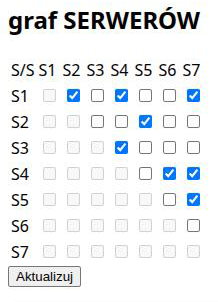
\includegraphics[width=0.3\textwidth]{materiały/screen1}
	\caption{Konfiguracja połączeń między serwerami}
\end{figure}

\vspace{15pt}
Na podstawie powyższej konfiguracji możemy uzyskać poniższy schemat połączeń:

\begin{figure}[H]
	\centering
	\vspace{15pt}
	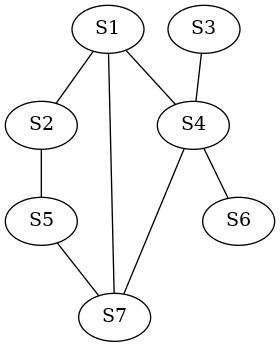
\includegraphics[width=0.35\textwidth]{materiały/screen2}
	\caption{Schemat połączeń}
\end{figure}

\newpage
\begin{empty}
	\begin{minted}[
		startinline,
		linenos,
		frame=lines,
		framesep=2mm,
		baselinestretch=1.2,
		fontsize=\footnotesize,
		breaklines,
		obeytabs=true,
		tabsize=2,
		]{php}
function convert_post_inputs_to_server_graph ()
{
	$graph = [];
	
	foreach ($_POST as $key => $val) {
		if (strpos($key, "connect_") === 0) {
			$pos = explode("_", $key);
			$pos = explode("x", $pos[1]);
			
			if (!isset($graph[$pos[0]])) {
				$graph[$pos[0]] = [];
			}
			
			$graph[$pos[0]][] = $pos[1];
		}
	}
	
	return (object) $graph;
}

function store_graph_configuration ($graph)
{
	file_put_contents("./graph.json", json_encode($graph));
}

function load_graph_configuration ()
{
	return json_decode(file_get_contents("./graph.json"));
}

if ($_SERVER['REQUEST_METHOD'] === 'POST' && $_POST['action'] == "graf") {
	$graph = convert_post_inputs_to_server_graph();
	store_graph_configuration($graph);
	cmd_broadcast([
		"action" => "graf",
		"graf" => $graph,
	]);
	log_msg("Zakutalizowano strukturę grafu");
}

$graph = load_graph_configuration();
	\end{minted}
	\captionof{listing}{Broadcast konfiguracji grafu do serwerów }
\end{empty}

\begin{empty}
	\begin{minted}[
		startinline,
		linenos,
		frame=lines,
		framesep=2mm,
		baselinestretch=1.2,
		fontsize=\footnotesize,
		breaklines,
		obeytabs=true,
		tabsize=2,
		]{json}
		{
			"1":["2", "4", "7"],
			"2":["5"],
			"3":["4"],
			"4":["6","7"],
			"5":["7"]
		}
	\end{minted}
	\vspace{-10pt}
	\captionof{listing}{Struktura grafu w formacie json}
\end{empty}

\vspace{10pt}
Graf ten rozgłaszany jest przez serwer centralny do mniejszych serwerów, serwery te odbierają go i zapisują sobie lokalne kopie w \textbf{/etc/graph.json}. Podczas ładowania struktura grafu jest rozwijana w drugą stronę tz. jeżeli serwer 3 widzi serwer 4, to w strukturze upewniamy się, że serwer 4 widzi też serwer 3.

\vspace{-10pt}
\begin{empty}
	\begin{minted}[
		startinline,
		linenos,
		frame=lines,
		framesep=2mm,
		baselinestretch=1.2,
		fontsize=\footnotesize,
		breaklines,
		obeytabs=true,
		tabsize=2,
		]{php}
function store_graph_configuration ($graph)
{
	file_put_contents("/etc/graph.json", json_encode($graph));
}

function load_graph_configuration ()
{
	$graph = (array) json_decode(file_get_contents("/etc/graph.json"));
	foreach ($graph as $key => $arr) {
		foreach ($arr as $val) {
			if (!isset($graph[$val])) {
				$graph[$val] = [];
			}
			if (!in_array($key, $graph[$val])) {
				$graph[$val][] = $key;
			}
		}
	}
	return $graph;
}

if ($_SERVER['REQUEST_METHOD'] === "POST" && $_POST['action'] === "graf") {
	store_graph_configuration($_POST['graf']); 
	exit;
}

$graph = load_graph_configuration();
	\end{minted}
	\vspace{-10pt}
	\captionof{listing}{Przejęcie grafu na serwerach}
\end{empty}


Kiedy serwery otrzymują polecenie o przesłaniu komunikatu do innego serwera, muszą one ustalić drogę, którą ten komunikat prześlą, innymi słowy, muszą ustalić, który z ich sąsiedzkich serwerów będzie mógł przekazać ten komunikat dalej. Poniżej znajduje się funkcja ustalająca taki serwer/drogę, jeżeli połączenie w grafie nie istnieje to serwer poddaje się zgłaszając serwerowi centralnemu stosowny komunikat. Algorytm nie szuka najbardziej optymalnej ścieżki, lecz pierwszej pasującej.

\begin{empty}
	\begin{minted}[
		startinline,
		linenos,
		frame=lines,
		framesep=2mm,
		baselinestretch=1.2,
		fontsize=\footnotesize,
		breaklines,
		obeytabs=true,
		tabsize=2,
		]{php}
$visited = [];

function route_graph_traverse ($ptr, $dest)
{
	global $graph;
	global $visited;
	$visited[] = $ptr;
	
	foreach ($graph[$ptr] as $edge) {
		
		if ($edge == $dest) {
			return $edge;
		}
		
		if (in_array($edge, $visited)) {
			/** już odwiedzony */
			continue;
		}
		
		if (route_graph_traverse($edge, $dest) != null) {
			return $edge;
		}
	}
	
	return null;
}

function route_graph ($dest)
{
	global $graph;
	global $serverId;
	return route_graph_traverse($serverId, $dest);
}
	\end{minted}
	\vspace{-10pt}
	\captionof{listing}{Trasowanie grafu}
\end{empty}

\newpage
\subsection{Logowanie operacji}
Istotną częścią projektu jest logowanie wszystkich operacji wykonywanych zarówno na serwerze centralnym jak i pomniejszych serwerach. 

\begin{figure}[H]
	\centering
	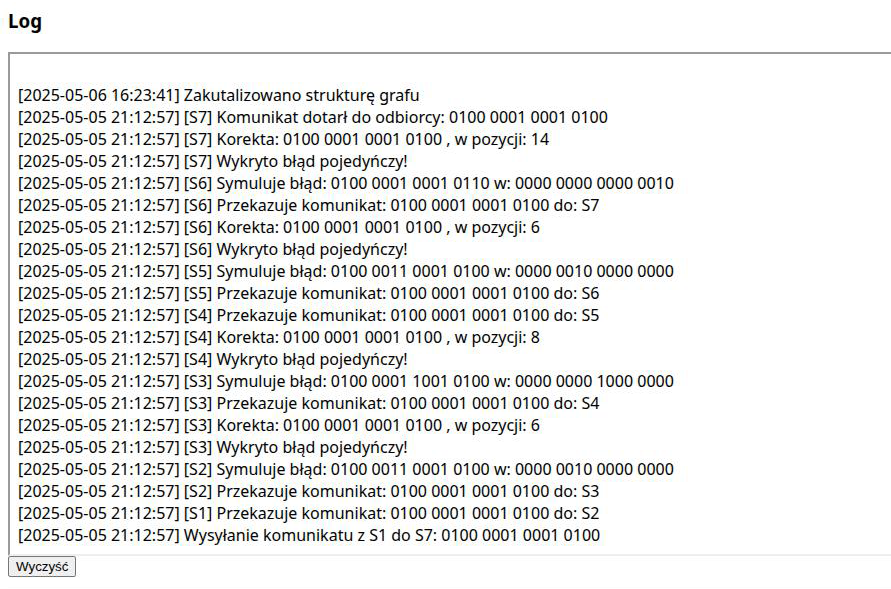
\includegraphics[width=0.8\textwidth]{materiały/screen3}
	\caption{Log widoczny dla użytkownika}
\end{figure}

Log przechowywany jest w pliku \textbf{log.txt}, na serwerze centralnym, jego wyświetlanie i automatyczne odświeżanie jest zrobione na zasadzie strony internetowej w \textbf{iframe}.

\begin{empty}
	\begin{minted}[
		startinline,
		linenos,
		frame=lines,
		framesep=2mm,
		baselinestretch=1.2,
		fontsize=\footnotesize,
		breaklines,
		obeytabs=true,
		tabsize=2,
		]{php}
<html>
	<head>
		<meta http-equiv="refresh" content="3">
	</head>
	<body>
	<?php
		$lines = explode("\n", file_get_contents("./log.txt"));

		for ($i = count($lines) - 1; $i >= 0; $i--) {
			echo $lines[$i] . "<br/>";
		}
	?>
	</body>
</html>
	\end{minted}
	\vspace{-10pt}
	\captionof{listing}{Wyświetlenie log'u}
\end{empty}

\newpage
\begin{empty}
	\begin{minted}[
		startinline,
		linenos,
		frame=lines,
		framesep=2mm,
		baselinestretch=1.2,
		fontsize=\footnotesize,
		breaklines,
		obeytabs=true,
		tabsize=2,
		]{php}
if ($_SERVER['REQUEST_URI'] === "/getlog") {
	include "./log.php";
	exit;
}

function msg_pp ($msg)
{
	return substr($msg, 0, 4) . " " . substr($msg, 4, 4) . " " . substr($msg, 8, 4) . " " . substr($msg, 12, 4);
}

function log_msg ($msg)
{
	file_put_contents("./log.txt", "[" . date('Y-m-d G:i:s') . "] " . $msg . "\n", FILE_APPEND);
}

if ($_SERVER['REQUEST_METHOD'] === "POST" && $_POST['action'] == "clear_log") {
	file_put_contents("./log.txt", "");
}

if ($_SERVER['REQUEST_METHOD'] === "POST" && $_POST['action'] == "log") {
	log_msg($_POST['msg']);
	exit;
}
	\end{minted}
	\vspace{-10pt}
	\captionof{listing}{Funkcje obsługujące log na serwerze centralnym}
\end{empty}

\begin{empty}
	\begin{minted}[
		startinline,
		linenos,
		frame=lines,
		framesep=2mm,
		baselinestretch=1.2,
		fontsize=\footnotesize,
		breaklines,
		obeytabs=true,
		tabsize=2,
		]{php}
function log_central ($msg)
{
	global $serverId;
	cmd_send([
		"action" => "log",
		"msg" => "[S{$serverId}] " . $msg
	], 0);
}
	\end{minted}
	\vspace{-10pt}
	\captionof{listing}{Funkcja umożliwiająca wysłanie log'a z pomniejszego serwera}
\end{empty}

\newpage
\subsection{Symulacja błędu}
Widok symulacji błędu jest załadowaną w iframe stroną serwera mniejszego, przyciski S1 do S7 zmieniają podgląd na konkretny serwer. Ustawienie konkretnego bitu sprawi, że w trakcie przekazywania komunikatu dalej przez ten serwer bit w ustawionej pozycji zostanie odwrócony, co pozwala w kontrolowany sposób symulować błędy. 


\begin{figure}[H]
	\centering
	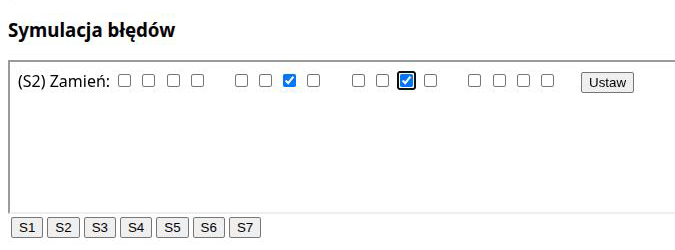
\includegraphics[width=0.7\textwidth]{materiały/screen4}
	\caption{Log widoczny dla użytkownika}
\end{figure}

\begin{empty}
	\begin{minted}[
		startinline,
		linenos,
		frame=lines,
		framesep=2mm,
		baselinestretch=1.2,
		fontsize=\footnotesize,
		breaklines,
		obeytabs=true,
		tabsize=2,
		]{php}
function toggler_sim ($msg, $bits)
{
	for ($i = 0; $i < 16; $i++) {
		if ($bits[$i] == '1') {
			$msg[$i] = ($msg[$i] == '1') ? '0' : '1';
		}
	}
	
	return $msg;
}

function store_toggler ($bits)
{
	file_put_contents("/etc/toggler.json", json_encode(["bits" => $bits]));
}

function load_toggler ()
{
	return json_decode(file_get_contents("/etc/toggler.json"))->bits ?? "0000000000000000";
}

if ($_SERVER['REQUEST_METHOD'] === "POST" && $_POST['action'] === "set") {
	$bits = "";
	
	for ($i = 0; $i < 16; $i++) {
		$bits .= isset($_POST["bit_{$i}"]) ? "1" : "0";
	}
	
	store_toggler($bits);
	log_central("S{$serverId} przestawia bity: " . msg_pp($bits));
}

$bits = load_toggler();

?>

<form action="/" method="POST">
	<input type="hidden" name="action" value="set" />

	(S<?= $serverId ?>) Zamień: 
	<? for ($i = 0; $i < 16; $i++): ?>
		<input type="checkbox" name="bit_<?= $i ?>" <?= $bits[$i] == "1" ? "checked" : "" ?> />
	
		<? if ($i % 4 == 3): ?>
			<span style="margin-left: 20px;"></span>
		<? endif ?>
	<? endfor ?>
	
	<button>Ustaw</button>
</form>
	\end{minted}
	\vspace{-10pt}
	\captionof{listing}{Obsługa symulacji błędów}
\end{empty}

\subsection{Wysłanie komunikatu}
Opcja wysłania komunikatu pozwala nam ustawić 11 bitów danych (pozostałe 5 to redundancja - bity parzystości). Pola do ustawiania bitów rozmieszczone są w wyglądzie macierzowym 4x4, z zaszarzonymi bitami parzystości - ich nie można ustawić. Ponadto możemy wybrać z którego do którego serwera komunikat ma zostać wysłany.

\begin{figure}[H]
	\centering
	\vspace{-10pt}
	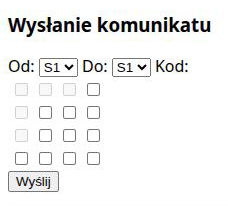
\includegraphics[width=0.3\textwidth]{materiały/screen5}
	\caption{Formularz do wysłania komunikatu}
\end{figure}

Po wysłaniu komunikatu wyświetla się podgląd macierzowy z obliczonymi bitami parzystości. 

\begin{figure}[H]
	\centering
	\vspace{-10pt}
	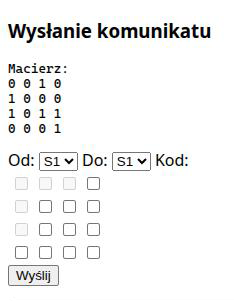
\includegraphics[width=0.35\textwidth]{materiały/screen6}
	\caption{Formularz do wysłania komunikatu}
\end{figure}

\begin{empty}
	\begin{minted}[
		startinline,
		linenos,
		frame=lines,
		framesep=2mm,
		baselinestretch=1.2,
		fontsize=\footnotesize,
		breaklines,
		obeytabs=true,
		tabsize=2,
		]{php}
    
if ($_SERVER['REQUEST_METHOD'] === "POST" && $_POST['action'] === "komunikat") {
	
	$hamming = [
		[0, 0, 0, 0],
		[0, 0, 0, 0],
		[0, 0, 0, 0],
		[0, 0, 0, 0],
	];
	
	for ($i = 0; $i < 4; $i++) {
		for ($j = 0; $j < 4; $j++) {
			$hamming[$i][$j] = isset($_POST["bit_{$i}x{$j}"]) ? 1 : 0;
		}
	}
	
	for ($i = 0; $i < 4; $i++) {
		$hamming[0][1] += $hamming[$i][1] + $hamming[$i][3];
		$hamming[0][2] += $hamming[$i][2] + $hamming[$i][3];
		
		$hamming[1][0] += $hamming[1][$i] + $hamming[3][$i];
		$hamming[2][0] += $hamming[2][$i] + $hamming[3][$i];
	}
	
	$hamming[0][1] %= 2;
	$hamming[0][2] %= 2;
	
	$hamming[1][0] %= 2;
	$hamming[2][0] %= 2;
	
	for ($i = 0; $i < 4; $i++) {
		for ($j = 0; $j < 4; $j++) {
			$hamming[0][0] += $hamming[$i][$j];
		}
	}
	
	$hamming[0][0] %= 2;
	\end{minted}
	\vspace{-10pt}
	\captionof{listing}{Obliczanie bitów parzystości}
\end{empty}

\vspace{20pt}
Tak przygotowany komunikat wysyłany jest do wybranego serwera, łącznie z informacją do którego serwera docelowo ma trafić. 

\begin{empty}
	\begin{minted}[
		startinline,
		linenos,
		frame=lines,
		framesep=2mm,
		baselinestretch=1.2,
		fontsize=\footnotesize,
		breaklines,
		obeytabs=true,
		tabsize=2,
		]{php}
	$msg = "";
	for ($i = 0; $i < 4; $i++) {
		for ($j = 0; $j < 4; $j++) {
			$msg .= $hamming[$i][$j] ? "1" : "0";
		}
	}
	
	log_msg("Wysyłanie komunikatu z S{$_POST['from']} do S{$_POST['to']}: " . msg_pp($msg));
	
	cmd_send([
		"action" => "komunikat",
		"to" => (int) $_POST['to'],
		"msg" => $msg
	], $_POST['from']);
		\end{minted}
		\vspace{-10pt}
		\captionof{listing}{Wysłanie komunikatu do wybranego serwera}
	\end{empty}
	
Serwer odbiera żądanie, weryfikuje poprawność komunikatu, jeżeli wystąpił błąd podwójny, to nie ma możliwości korekcji, na serwer centralny wysyłana jest stosowna informacja. Jeżeli wystąpił błąd pojedynczy to jest on korygowany. Dalej jeżeli serwer jest odbiorcą to przesyłanie zakańcza się, jeżeli nie to wyznaczana jest trasa, dokonywana jest ewentualna symulacja błędu, komunikat przekazywany jest do kolejnego węzła w grafie.  

\newpage
\begin{empty}
	\begin{minted}[
		startinline,
		linenos,
		frame=lines,
		framesep=2mm,
		baselinestretch=1.2,
		fontsize=\footnotesize,
		breaklines,
		obeytabs=true,
		tabsize=2,
		]{php}
if ($_SERVER["REQUEST_METHOD"] === "POST" && $_POST['action'] === "komunikat") {
	
	$msg = $_POST['msg'];
	
	/** Sprawdzeneie czy komuniakt posiada błąd */
	$msg = hamming_check($msg);
	if ($msg === false) {
		exit;
	}
	
	if ($_POST['to'] == $serverId) {
		/** Jesteśmy odbiorcą! */
		log_central("Komunikat dotarł do odbiorcy: " . msg_pp($msg));
		exit;
	}
	
	$route = route_graph($_POST['to']);
	
	if ($route == null) {
		/** Droga nie istnieje */
		log_central("Droga do S{$_POST['to']} przez S{$serverId} nie istnieje!");
		exit;
	}
	
	log_central("Przekazuje komunikat: " . msg_pp($msg) . " do: S{$route}");
	
	/** Symulacja błędu na podstawie ustawień */
	$bits = load_toggler();
	if (strpos($bits, "1") !== false) {
		$msg = toggler_sim($msg, $bits);
		log_central("Symuluje błąd: " . msg_pp($msg) . " w: " . msg_pp($bits));
	}
	
	/** Przekazujemy komunikat do kolejnego serwera */
	cmd_send([
		"action" => "komunikat",
		"msg" => $msg,
		"to" => $_POST['to']
	], (int) $route);
	
	exit;
}
	\end{minted}
	\vspace{-10pt}
	\captionof{listing}{Obsługa komunikatu przez serwery}
\end{empty}

Funkcja \textbf{hamming\_check()} sprawdzająca, korygująca komunikat i zwracająca prawidłowy komunikat lub NULL w przypadku błędu podwójnego.

\begin{empty}
	\begin{minted}[
		startinline,
		linenos,
		frame=lines,
		framesep=2mm,
		baselinestretch=1.2,
		fontsize=\footnotesize,
		breaklines,
		obeytabs=true,
		tabsize=2,
		]{php}
function hamming_check ($msg)
{
	/** OMP */
	$omp = 0;
	for ($i = 0; $i < 16; $i++) {
		$omp += $msg[$i] == '1' ? 1 : 0;
	}
	$omp %= 2;
	
	$mx = [
		[0, 0, 0, 0],
		[0, 0, 0, 0],
		[0, 0, 0, 0],
		[0, 0, 0, 0]
	];
	
	for ($i = 0; $i < 4; $i++) {
		for ($j = 0; $j < 4; $j++) {
			$mx[$i][$j] = ($msg[$i * 4 + $j] == '1') ? 1 : 0;
		}
	}
	
	/**
	* Liczenie bitów parzystości, i sprawdzenie z orginalnymi
	* oraz z dodatkowym w celu określenia ilości błędów, i 
	* ewentualnej możliwości korekty
	*/
	
	$op1 = $mx[0][1];
	$op2 = $mx[0][2];
	$op4 = $mx[1][0];
	$op8 = $mx[2][0];
	
	$mx[0][1] = 0;
	$mx[0][2] = 0;
	$mx[1][0] = 0;
	$mx[2][0] = 0;
	
	$p1 = 0;
	$p2 = 0;
	$p4 = 0;
	$p8 = 0;
	
	for ($i = 0; $i < 4; $i++) {
		$p1 += $mx[$i][1] + $mx[$i][3];
		$p2 += $mx[$i][2] + $mx[$i][3];
		
		$p4 += $mx[1][$i] + $mx[3][$i];
		$p8 += $mx[2][$i] + $mx[3][$i];
	}
	
	$p1 %= 2;
	$p2 %= 2;
	$p4 %= 2;
	$p8 %= 2;
	
	$areParityBitsCorrect = ($p1 == $op1 && $p2 == $op2 && $p4 == $op4 && $p8 == $op8);
	$isOveralParityCorrect = $omp == 0;
	
	/** Nie da się poprawić, dwa błędy */
	if (!$areParityBitsCorrect && $isOveralParityCorrect) {
		log_central("Wykryto błąd podwójny, poddaje się!");
		return false;
	}
	
	/** Nie ma co porpawiać, parzystość się zgadza */
	if ($areParityBitsCorrect && $isOveralParityCorrect) {
		return $msg;
	}
	
	log_central("Wykryto błąd pojedyńczy!");
	
	/**
	* Jak weźmiemy {p8, p4, p2, p1}, to jest to
	* dosłownie index bitu który był flipnięty
	*/
	
	$pos = "0000";
	
	if ($p1 != $op1) {
		$pos[3] = '1';
	}
	
	if ($p2 != $op2) {
		$pos[2] = '1';
	}
	
	if ($p4 != $op4) {
		$pos[1] = '1';
	}
	
	if ($p8 != $op8) {
		$pos[0] = '1';
	}
	
	$pos = bindec($pos);
	$msg[$pos] = ($msg[$pos] == '1') ? '0' : '1';
	
	log_central("Korekta: " . msg_pp($msg) . " , w pozycji: " . $pos);
	
	return $msg;
}

	\end{minted}
	\vspace{-10pt}
	\captionof{listing}{Funkcja implementująca sprawdzanie i korekcję Hamminga}
\end{empty}

\begin{figure}[H]
	\centering
	\vspace{-10pt}
	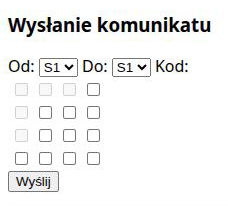
\includegraphics[width=0.3\textwidth]{materiały/screen5}
	\caption{Formularz do wysłania komunikatu}
\end{figure}

\begin{empty}
	\begin{minted}[
		startinline,
		linenos,
		frame=lines,
		framesep=2mm,
		baselinestretch=1.2,
		fontsize=\footnotesize,
		breaklines,
		obeytabs=true,
		tabsize=2,
		]{text}
Wysyłanie komunikatu z S7 do S1: 0000 0000 0000 0000
[S7] Przekazuje komunikat: 0000 0000 0000 0000 do: S6
[S7] Symuluje błąd: 0001 0000 0000 0000 w: 0001 0000 0000 0000
[S6] Wykryto błąd pojedyńczy!
[S6] Korekta: 0000 0000 0000 0000 , w pozycji: 3
[S6] Przekazuje komunikat: 0000 0000 0000 0000 do: S5
[S6] Symuluje błąd: 0000 0000 0000 0010 w: 0000 0000 0000 0010
[S5] Wykryto błąd pojedyńczy!
[S5] Korekta: 0000 0000 0000 0000 , w pozycji: 14
[S5] Przekazuje komunikat: 0000 0000 0000 0000 do: S4
[S5] Symuluje błąd: 0000 0010 0000 0000 w: 0000 0010 0000 0000
[S4] Wykryto błąd pojedyńczy!
[S4] Korekta: 0000 0000 0000 0000 , w pozycji: 6
[S4] Przekazuje komunikat: 0000 0000 0000 0000 do: S3
[S3] Przekazuje komunikat: 0000 0000 0000 0000 do: S2
[S3] Symuluje błąd: 0000 0000 1000 0000 w: 0000 0000 1000 0000
[S2] Wykryto błąd pojedyńczy!
[S2] Korekta: 0000 0000 0000 0000 , w pozycji: 8
[S2] Przekazuje komunikat: 0000 0000 0000 0000 do: S1
[S2] Symuluje błąd: 0000 0010 0000 0000 w: 0000 0010 0000 0000
[S1] Wykryto błąd pojedyńczy!
[S1] Korekta: 0000 0000 0000 0000 , w pozycji: 6
[S1] Komunikat dotarł do odbiorcy: 0000 0000 0000 0000
	\end{minted}
	\vspace{-10pt}
	\captionof{listing}{Przebieg komunikacji między S7 i S1 z pustym komunikatem}
\end{empty}

\begin{empty}
	\begin{minted}[
		startinline,
		linenos,
		frame=lines,
		framesep=2mm,
		baselinestretch=1.2,
		fontsize=\footnotesize,
		breaklines,
		obeytabs=true,
		tabsize=2,
		]{text}
Wysyłanie komunikatu z S1 do S7: 0100 0001 0001 0100
[S1] Przekazuje komunikat: 0100 0001 0001 0100 do: S2
[S1] Symuluje błąd: 0100 0101 0001 0100 w: 0000 0100 0000 0000
[S2] Wykryto błąd pojedyńczy!
[S2] Korekta: 0100 0001 0001 0100 , w pozycji: 5
[S2] Przekazuje komunikat: 0100 0001 0001 0100 do: S3
[S2] Symuluje błąd: 0100 0011 0001 0100 w: 0000 0010 0000 0000
[S3] Wykryto błąd pojedyńczy!
[S3] Korekta: 0100 0001 0001 0100 , w pozycji: 6
[S3] Przekazuje komunikat: 0100 0001 0001 0100 do: S4
[S3] Symuluje błąd: 0100 0001 1001 0100 w: 0000 0000 1000 0000
[S4] Wykryto błąd pojedyńczy!
[S4] Korekta: 0100 0001 0001 0100 , w pozycji: 8
[S4] Przekazuje komunikat: 0100 0001 0001 0100 do: S5
[S5] Przekazuje komunikat: 0100 0001 0001 0100 do: S6
[S5] Symuluje błąd: 0100 0011 0001 0100 w: 0000 0010 0000 0000
[S6] Wykryto błąd pojedyńczy!
[S6] Korekta: 0100 0001 0001 0100 , w pozycji: 6
[S6] Przekazuje komunikat: 0100 0001 0001 0100 do: S7
[S6] Symuluje błąd: 0100 0001 0001 0110 w: 0000 0000 0000 0010
[S7] Wykryto błąd pojedyńczy!
[S7] Korekta: 0100 0001 0001 0100 , w pozycji: 14
[S7] Komunikat dotarł do odbiorcy: 0100 0001 0001 0100
	\end{minted}
	\vspace{-10pt}
	\captionof{listing}{Przebieg komunikacji między S1 i S7 z testowym komunikatem}
\end{empty}

\newpage
\begin{empty}
	\begin{minted}[
		startinline,
		linenos,
		frame=lines,
		framesep=2mm,
		baselinestretch=1.2,
		fontsize=\footnotesize,
		breaklines,
		obeytabs=true,
		tabsize=2,
		]{text}
[S4] S4 przestawia bity: 0000 1100 0000 0000
Wysyłanie komunikatu z S1 do S7: 1101 1000 1110 0100
[S1] Przekazuje komunikat: 1101 1000 1110 0100 do: S2
[S1] Symuluje błąd: 1101 1100 1110 0100 w: 0000 0100 0000 0000
[S2] Wykryto błąd pojedyńczy!
[S2] Korekta: 1101 1000 1110 0100 , w pozycji: 5
[S2] Przekazuje komunikat: 1101 1000 1110 0100 do: S3
[S2] Symuluje błąd: 1101 1010 1110 0100 w: 0000 0010 0000 0000
[S3] Wykryto błąd pojedyńczy!
[S3] Korekta: 1101 1000 1110 0100 , w pozycji: 6
[S3] Przekazuje komunikat: 1101 1000 1110 0100 do: S4
[S3] Symuluje błąd: 1101 1000 0110 0100 w: 0000 0000 1000 0000
[S4] Wykryto błąd pojedyńczy!
[S4] Korekta: 1101 1000 1110 0100 , w pozycji: 8
[S4] Przekazuje komunikat: 1101 1000 1110 0100 do: S5
[S4] Symuluje błąd: 1101 0100 1110 0100 w: 0000 1100 0000 0000
[S5] Wykryto błąd podwójny, poddaje się!
	\end{minted}
	\vspace{-10pt}
	\captionof{listing}{Przebieg komunikacji między S1 i S7 z podwójnym błędem}
\end{empty}
